\documentclass{article}
\usepackage{FinalYearProjectReport}

\sloppy

% packages and settings for graphics
\usepackage[pdftex]{graphicx}
\usepackage{booktabs}
\graphicspath{{./}}
\DeclareGraphicsExtensions{.png}
\usepackage[final]{pdfpages}

\setlength\paperheight{297mm}
\setlength\paperwidth{210mm}

\usepackage{avant}
\renewcommand{\familydefault}{\sfdefault}
\frenchspacing

\title{Final Report}
\name{Alex \textsc{Andela}, Adil \textsc{Bhayani}, Vaishnavi \textsc{Muppavaram} \& Sakayan \textsc{Sitsabesan}}
\address{Department of Electrical and Computer Engineering\\
University of Auckland, Auckland, New Zealand}

\begin{document}

\begin{titlepage}

\newcommand{\HRule}{\rule{\linewidth}{0.5mm}}

\center
 
%----------------------------------------------------------------------------------------
%	HEADING SECTIONS
%----------------------------------------------------------------------------------------

\textsc{\LARGE University of Auckland}\\[1.5cm]
\textsc{\Large COMPSYS 301: Design: Hardware and Software Systems }\\[0.5cm]
\textsc{\large Autonomous Line Following Robot}\\[0.5cm]

%----------------------------------------------------------------------------------------
%	TITLE SECTION
%----------------------------------------------------------------------------------------

\HRule \\[0.4cm]
{ \huge \bfseries Final Report}\\[0.4cm]
\HRule \\[1.5cm]
 
%----------------------------------------------------------------------------------------
%	AUTHOR SECTION
%----------------------------------------------------------------------------------------

\begin{minipage}{0.4\textwidth}
\begin{flushleft} \large
\emph{Authors:}\\
Alex \textsc{Andela} \newline
Adil \textsc{Bhayani} \newline
Vaishnavi \textsc{Muppavaram} \newline
Sakayan \textsc{Sitsabesan}
\end{flushleft}
\end{minipage}
~
\begin{minipage}{0.4\textwidth}
\begin{flushright} \large
\emph{Supervisors:} \\
Dr. Nitish \textsc{Patel} \\
Dr. Muhammad \textsc{Nadeem} % Supervisor's Name
\end{flushright}
\end{minipage}\\[1cm]

%----------------------------------------------------------------------------------------
%	DATE SECTION
%----------------------------------------------------------------------------------------

{\large \today}\\[2cm]

%----------------------------------------------------------------------------------------
%	LOGO SECTION
%----------------------------------------------------------------------------------------


\includegraphics{uoa.png}\\[1cm]
 
%----------------------------------------------------------------------------------------

\vfill

\vspace*{25em}

{\Large Declaration of Originality}

\hspace{5em}

This report is our own unaided work and was not copied from nor written in collaboration with any other person.

Name: Alex \textsc{Andela}, Adil \textsc{Bhayani}, Vaishnavi \textsc{Muppavaram} \& Sakayan \textsc{Sitsabesan}

\newpage

{\Large Acknowledgments}

\hspace{5em}

We would like to thank our supervisors, Dr. Nitish Patel \& Dr. Muhammad Nadeem, for guiding us throughout the semester with their constant help, supervision and suggestions. We would also like to thank Fung Yang \& Howard Lu for their patience dealing with our numerous issues and changes with the robot hardware. Special mentions need to be made to Joseph Tsoi, Andrew Lai \& John Zhang for their ideas and assistance.

\end{titlepage}

\newpage

\maketitle

%----------------------------------------------------------------------------------------
%	ABSTRACT
%----------------------------------------------------------------------------------------

\begin{abstract}

The Mini Project consists of designing a game on a FPGA device which incorporates one simple tank defence game called Tank Hunting. The overall objective is to learn the process of digital design and logic by practically applying the skills learnt prior to the project.

\end{abstract}

%----------------------------------------------------------------------------------------
%	INTRODUCTION
%----------------------------------------------------------------------------------------

\section{Design Overview}

This project consisted of the design and construction of part of an autonomous line following robot, which will complete certain benchmarks and can pick up all the "food pellets" in a given map. Much of the robot's hardware was prescribed and given to us in an assembled state for working on. The sensor circuit was the only important part of the hardware that needed to be completed as part of this project. The robot was controlled from a Cypress PSoC 5LP, which interfaced with the Sensors, RF, Bluetooth \&  Motors to allow the robot to meet its requirements. This report outlines the hardware and software considerations and decisions that were made as part of this project.

\section{Robot Description}

%----------------------------------------------------------------------------------------
%	ANALOGUE SECION
%----------------------------------------------------------------------------------------
% Mention considerations and decisions here

\section{Analogue}

The portion of the hardware that needed to be developed as part of this project centred around the collection and processing of vision information. This was in the form of a surface mounted phototransistor, the TEMT6200. The map is projected down from a ceiling mounted projector, where black lines represent lines and white areas symbolizes the walls. To be able to sense the difference between these and convey this information on to the PSoC is the aim of the analogue section of this project.

\subsection{Phototransistor output signal}

The phototransistor can be configured in two ways: common emitter or common collector. In the common emitter configuration, the output signal was very flat $(Black: V_{avg} = 2.58V, V_{Pk-Pk} = 0.05V, White: V_{avg} = 2.74V, V_{Pk-Pk} = 0.10V)$ and difficult to differentiate between the black and white lines. On the other hand in the common collector configuration, there was a sharp difference between the black and white lines $(Black: V_{avg} = 4.09V, V_{Pk-Pk} = 0.09V, White: V_{avg} = 2.84V, V_{Pk-Pk} = 1.54V)$. As a result a decision was made to use the common collector configuration for the light sensors.

\subsection{Circuitry}

There are two main concerns in the phototransistor output signal that must be resolved by the circuitry; these being the removal of the DC offset in the signal, and the filtering of noise. The DC offset needed to be removed as this varied depending on projector brightness in various parts of the map \& external lighting. The projector to be used for this project has a refresh rate of 120Hz, while the ambient light source in the laboratory has a refresh rate of 100Hz. Therefore a High pass filter with a cut-off less than 120Hz is necessary for this project. In this regard, the group's decision was to implement a RC High Pass filter with a cut-off frequency of 106Hz.

The next thing that needed to be considered was how the signal will be passed onto the PSoC, in digital or analogue form. If the signal were to be passed on as a analogue signal, the PSoC must sample the signal and process this into a binary output (black or white) at a fast enough rate for the robot to accurately follow the line. Alternatively a hardware Schmitt Trigger can be used on the output signal to create a digital binary output which can be read by the PSoC from one of it's digital pins. This solution process the information into what is relevant to us in real time. After much thought and weighting of the pros and cons, a decision was reached to  use a Schmitt Trigger and process the signal into a digital signal to be passed into the PSoC.

\subsection{Light sensor array and robot orientation}

The project requires a sensor circuit layout such that it can communicate as much information as possible about the current position of the robot to the PSoC, so that the robot can interpret the track well to make an informed decision on where to move to next. After doing much research into the intricacies of line following robots, it became apparent that a line could be followed with as few as two sensors.

One sensor immediately on either side of the inside of the line is sufficient to track a line and follow it. These two sensors must be placed as far forward as possible so as to make the deviations of the robot more pronounced and easier to detect \& correct. This would result in the robot being able to follow the lines more smoothly and jerk a lot less than if the sensors were near the axis of the wheels.

In our project it is not sufficient for the robot to follow a line, it must also be able detect intersections and take 90° turns. For this purpose two addition sensors were used, these were placed on either side of the line slightly behind the front two sensors. These were placed forward so that when an intersection is detected by these sensors, there is enough of a braking distance for the robot to brake in time to take a turn at the intersection.

\subsection{PCB Design}

An important decision that needed to made with regards to the PCB design was the use of through-hole mounted (THM) or Surface Mounted Devices (SMD) components.

The use of through hole components allows us to rapidly prototype the board, with ease of switching out components after assembly. As the component leads run through the board and soldered over a larger surface area, through-hole mounted circuit boards offer higher reliability and stronger connections. This is very important in cases where there are extreme accelerations, collisions or high temperatures.

Surface mount technology does not require holes to be drilled through the board, are much smaller, can be automatically placed and can be mounted on both sides of the board. This usually leads to a smaller designs, higher component density, lower cost and faster assembly times. 

In this project, higher reliability and extreme environmental conditions are not of major concern. But the benefits of surface mount technology allowed a quicker design and assembly time for this project. Both sides of this decision were carefully considered and the group came to a decision of going with the use of SMD components.

Other considerations for the PCB design were the routing of the pins to the PSoC, whether the H-Bridges will be connected via traces and the presence of switches for easy operation. The pin assignments to be used for routing the pins to the PSoC were very carefully planned and executed. Much consideration was put into reducing track lengths and making certain that only usable pins were used.

Two bi-polar switches that are easy to operate were used as a power on/off switch for the board and localization LEDs. These were used as it allowed both the PCB and the localization LEDs to be individually turned on and off, this was important when sharing the maze with other groups' robots without interference. In addition two 2-DIP switches were added to enable easy switching between the various modes and configurations of the robot.

Connecting the H-bridges via traces would result in a cleaner design with no rogue wires, but would come at the expense of having more long pins connecting the PCB to the daughterboard, which would cause headaches when assembling the two together. A decision was taken to connect via traces as we realized that the board need not be connected together many times and that this little inconvenience was well worth the much tidier robot connections.

\subsection{Testing and Verification}

\subsection{Final Design}

%----------------------------------------------------------------------------------------
%	DIGITAL SECION
%----------------------------------------------------------------------------------------
% Mention considerations and decisions here

\section{Digital}

\subsection{Path Finding Algorithms}

There are numerous ways to find the shortest path to a particular location in a maze, of these we considered the Depth First Search (DFS) \& A* algorithms.

When trying to reach the target, DFS navigates by following a path till the depth is reached, then traverse backwards till the previous intersection then choosing the next undiscovered path. A maze can be modelled as a tree with nodes in it. Each intersection can be considered a node. This can be implemented using recursion or iteration. There are few issues with this method: it doesn't find the shortest path, if loops exist additional making is necessary to solve, often suboptimal performance because it doesn't prioritise direction based on goal.

On the other hand the A* algorithm is a much better transversal algorithm in most cases. Given a start \& end, A* prioritises which nodes to discover by using heuristic to estimate how far node is from goal. It then continues the search from the it thinks is closest to the goal. We have decided to use the Manhattan heuristic in our implementation. Manhattan distance is the distance between in a grid assuming strictly horizontal or vertical movements and the absence of objects. Often in multipath mazes where there is more than one path to the destination, finding the shortest path can take longer due to backtracking. Sometimes it is better to continue on a chosen path then to travers back a large distance to get the shortest path.

\subsection{Line Following}

\subsection{Motion Control \& PID}

\subsection{RF \& Bluetooth}

RF and Bluetooth are two methods of wireless communication that the robot can interface with. With RF communication, the serial stream coming from the projector control computer can be received as in binary form as a C Struct or a space separated ASCII string. The ASCII string is human readable and easier to work with initially. The processing time required to convert this into something usable is much greater than for receiving and storing the binary C Struct. The coding required to achieve this is more tedious and repetitive but much easier than the binary method. As a result of weighing both sides, we decided to use the binary form C Struct method of RF reception.

The Bluetooth module used enabled bi-direction wireless communication between the robot and a computer. This present numerous oppurtunities, a few of which were explored in this project. The possibility of Bluetooth boot loading the PSoC was on of the more ambitious ideas that was considered. After setting this up, it was found that it took 45+ seconds to download the program to the PSoC over Bluetooth and it was prone to cut-outs due to signal loss. Due to this, this possibility was not explored any further and was not used in the final project.

Other uses of the Bluetooth module including passing in input arguments for particular modes of operations, outputting status information about the robot and using this as a channel for debugging. These options were well used and were critical to saving a lot of development time and keeping the final project flexible.

\subsection{Testing and Verification}

\subsection{Final Design}

\subsection{Data Structures}

%----------------------------------------------------------------------------------------
%	CONCLUSIONS
%----------------------------------------------------------------------------------------

\section{Conclusions}

\clearpage

\section{Contributions}

\begin{table}[h]
\centering
\label{my-label}
\begin{tabular}{@{}l|cccc@{}}
\toprule
Task                          & \multicolumn{1}{l}{Alex Andela} & \multicolumn{1}{l}{Adil Bhayani} & \multicolumn{1}{l}{Vaishnavi Muppavaram} & \multicolumn{1}{l}{Sakayan Sitsabesan} \\ \midrule
Analogue Design               & 40\%                            & 0\%                              & 50\%                                     & 10\%                                   \\
Analogue Testing              & 50\%                            & 0\%                              & 40\%                                     & 10\%                                   \\
Hardware Assembly             & 0\%                             & 10\%                             & 30\%                                     & 60\%                                   \\
PID Control                   & 0\%                             & 40\%                             & 0\%                                      & 60\%                                   \\
Matlab Algorithm              & 0\%                             & 100\%                            & 0\%                                      & 0\%                                    \\
Pacman Algorithms             & 30\%                            & 40\%                             & 30\%                                     & 0\%                                    \\
Benchmark Tasks               & 20\%                            & 30\%                             & 20\%                                     & 30\%                                   \\
Project Archiving             & 55\%                            & 5\%                              & 25\%                                     & 15\%                                   \\
Integration & 30\%                            & 0\%                              & 30\%                                     & 40\%                                   \\ \bottomrule
\end{tabular}
\end{table}

%----------------------------------------------------------------------------------------
%	APPENDICES
%----------------------------------------------------------------------------------------

\clearpage

\section{Appendices}

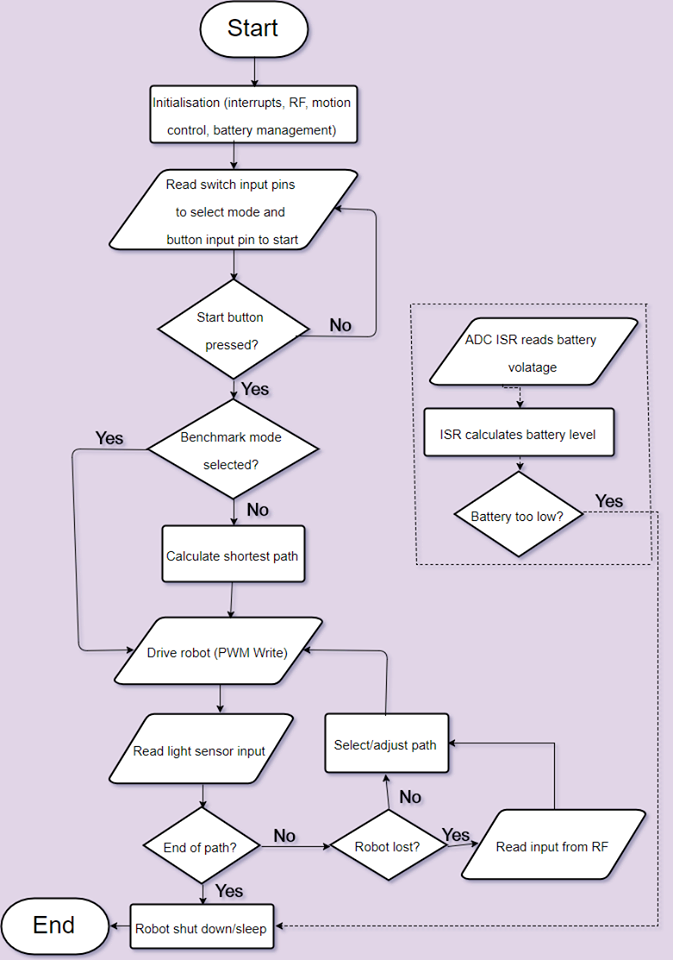
\includegraphics[width=0.5\textwidth]{software_flowchart.png}

\vfill

\end{document}